%
% CHAPTER 6.- The Theory of Nescience
%

% TODO: Review that we always say "we define" instead of "it is defined"
% TODO: We promised to prove that \sigma(d_{t,s} \geq \sigma{d_t}

%
%  Section 1:
%    - (2nd)   How Shannon's entropy and nescience relates?
%    - (2nd)   Plot nescience. Is it concave or convex?
%    - (2nd)   How the complexity of a topic relates to randomness 
%  Section 2:
%    - TODO:   Talk about prefix-free string
%

\chapterimage{owl.pdf} % Chapter heading image

\chapter{Nescience}
\label{chap:Nescience}

\begin{quote}
\begin{flushright}
\emph{There are known knowns. These are things we know that we know.
There are known unknowns. That is to say, there are things that we know we don't know.
But there are also unknown unknowns. There are things we don't know we don't know.} \\
Donald Rumsfeld
\end{flushright}
\end{quote}
\bigskip

After a preliminary Chapter \ref{cha:Topics-and-Descriptions}, in which we formally defined the concepts of entity, representation, and description, and subsequent Chapters \ref{chap:Miscoding}, \ref{chap:Error} and \ref{chap:Redundancy}, where we introduced new metrics for miscoding, inaccuracy, and surfeit, we now have all the necessary elements to delve into the critical concept of nescience in this chapter and examine its primary properties.

Nescience, on the contrary of what happens with the entropy of Shannon or the complexity of Kolmogorov, is not a measure of the quantity of information; instead, what it measures is the lack of information, that is, the unknown. According to the theory of nescience, how much we do not know about a research entity is given by the three new metrics studied: miscoding, inaccuracy and surfeit. Miscoding measures how good is the representation of the original entity as a string of symbols that we can use in our research; inaccuracy measures how well our current best model describe that string of symbols; and sufeit measures how well we understand the description itself, based on the length, or number of symbols, of the model. The problem of these quantities is that they are conflicting, in the sense that decreasing one of them could increase the other two. We have to find a way to minimize all of them at the same time, that is, science is a multiobjective minimization problem.

One of the most important consequences of our definition of nescience, based on the metrics of miscoding, inaccuracy and surfeit, is that it divides the space of research topics into two different areas. The first area is what we call the known unknown, that is, the set of topics that we do not fully understand, but that we are aware that we do non fully understand them. The second area is the unknown unknown, composed by those topics that have not been discovered yet. An inportant application of the theory of nescience is as a methodology for the discovery of what hides in the unknown unknown. A second important consequence of the concept of nescience is the highly counterintuitive property that sometimes, for a certain class of topics, further research could be a counterproductive activity. That is, the more research we do, the less we know, since for these topics it is not possible to increase our knowledge beyond a critical point, even if this point we are far from having a perfect knowledge.

%
% Section: Nescience
%

\section{Nescience}

Intuitively, how much we do not know about a topic should be based on the quality of the model we are using to describe it, that is, its capacity to eplain why things happen. In the theory of nescience we propose to quantitatively measure how much we do not know about a research entity using the misscoding of a string-based representation of the entity, and the inaccuracy and surfeit of the model describing this representation. Miscoding because it tells us how good the representation is at encoding the entity, inaccuracy since it measures how close our model is to adequately describe the representation, and surfeit to quantify how much unnecessary effort we are putting into the model. We believe that the goal of Science should be to minimize these three quantities: miscoding, inaccuracy and surfeit. Unfortunately they are conflicting metrics, in the sense that decreasing one of them could increase the other two.

According to the theory of nescience, science is about solving the following multiobjective optimization problem\footnote{Thechnically speaking science is a deterministic discrete nonlinear nonconvex nondifferentiable multiobjective optimizaton problem with a single decision maker.}:

\begin{tBox}
\textbf{The Science Problem}
\begin{align*}
 & \text{minimize} \quad \{ \mu(r), \iota(d, r), \sigma(d, r)\} \\
 & \text{subject to} \quad (r, d) \in \mathcal{B}^\ast \times \mathcal{D}
\end{align*}
\end{tBox}

A \emph{scientific mehtod} (see Section \ref{sec:scientific_method}) would be any computable procedure to solve the above minimization problem.

The feasible region is the cartesian product $\mathcal{B}^\ast \times \mathcal{D}$ of the set of finite binary strings $\mathcal{B}^\ast$ and the set of descriptions $\mathcal{D}$, the decision vectors are pairs $(r, d)$ composed by a representation and a description, and the objective functions to minize are miscoding, surfeit and inaccuracy. The objective region is a subset of $\mathbf{Z} \subset \mathbb{R}^3$ and its elements are the objective vectors.

In our characterization of science and the scientific method we do not involve the set $\mathcal{E}$ of entities, since requiring to know the entity $e \in \mathcal{E}$ under study would make science an ill-defined problem for the majority of the research areas. Science is basically a problem of manipulating strings of symbols. From a practical point of view, science is about finding strings that have a meaningful intepretation in the real world, and that allow us to solve practical problems. From a more theoretical point of view, the goal of science would be to understand how a unknown abstract oracle works.

If the set $\mathcal{R}_e$ of representations of the particular entity $e$ in which we are interested is known, or approximately known, we could restrict the science problem to:
\begin{align*}
 & \text{minimize} \quad \{ \mu(r), \iota(d, r), \sigma(d, r)\} \\
 & \text{subject to} \quad (r, d) \in \mathcal{R}_e \times \mathcal{D}
\end{align*}
In the theory of nescience we are mostly interested in the decision space $\mathcal{B}^\ast \times \mathcal{D}$ of respresentations and descriptions reather than in the objective space $\mathbf{Z} \subset \mathbb{R}^3$ of metric values. In the following definitions we re-introduce some of the concepts of multiobjective optimization (see Section \ref{sec:multiobjective_optimization}) for the particular case of the science problem.

If the representation and description currently in use are not perfect, our goal is to find another representation, or another description, that reduces at least one of the metrics miscoding, inaccuracy or surfeit without deteriorating either of the other two.

\begin{definition}
We say that a decision vector $(r, d) \in \mathcal{B}^\ast \times \mathcal{D}$ \emph{dominates} another decision vector $(r', d') \in \mathcal{B}^\ast \times \mathcal{D}$ if it improves in one of the metrics miscoding, inaccuracy or surfeit without deteriorating either of the other two.
\end{definition}

For the majority of the applications, it does not exists a single solution that simultaneously minimize the three metrics. Instead, what we have is a collection of Pareto optimal solutions that define an optimal frontier.

\begin{definition}
We say that a decision vector $(r, d) \in \mathcal{B}^\ast \times \mathcal{D}$ is \emph{Pareto optimal} if there does not exists another decision vector $(r', d') \in \mathcal{B}^\ast \times \mathcal{D}$ such that $(r', d')$ dominates $(r, d)$. The set of Pareto optimal solutions, denoted by $\mathbf{P}_{\mathcal{B}^\ast \times \mathcal{D}}$, is called the \emph{Pareto frontier}.
\end{definition}

The concepts of dominiation and Pareto optimality can be defined in the same way for the restricted decision space $\mathcal{R}_e \times \mathcal{D}$.

In general, weakly Pareto optimal solutions are not relevant in the theory of nescience. {\color{red} Explain why.}

% Range of Solutions

\subsection{Range of Solutions}

As we have seen in Section \ref{sec:range_solutions}, an objective vector that minimizes all objective functions is called an ideal objective vector. In case of the science problem, the ideal objective vector is the origin $(0, 0, 0)$, in which we have zero miscoding, zero inaccuracy and zero surfeit.

\begin{proposition}
The ideal objective vector of the Science Problem is the origin $(0, 0, 0)$.
\end{proposition}
\begin{proof}
{\color{red} TODO}
\end{proof}

A decision vector $(r, d) \in \mathcal{B}^\ast \times \mathcal{D}$ is ideal if it has zero miscoding, zero inaccuracy and zero surfeit. That is, the representation $r$ is {\color{red}valid}, the output of the model $d$ is $r$, and it does not exist another shorter model $d'$ with zero inaccuracy. Intuitively, a decision vector $(r, d)$ is ideal if there exists an enty $e \in \mathcal{E}$, such that $r$ perfectly encodes $e$, and the model $d$ of $r$ is accurate and minimal. Ideal decision vectors represent the concept of perfect knowledge in the theory of nescience.

{\color{red} Introduce the following proposition.}

\begin{proposition}
Let $(r, d) \in \mathcal{B}^\ast \times \mathcal{D}$ be an ideal decision vector, then $d$ must be a random string.
\end{proposition}
\begin{proof}
{\color{red} TODO}
\end{proof}

The upper bound of the Pareto optimal set is given by the nadir objective vector. In the theory of nescience, the nadir vector would be the $(1, 1, 1)$ vector, in which we have the maximum miscoding, minimal accuracy, and maximun surfeit.

\begin{proposition}
The nadir objective vector of the Science Problem is the vector $(1, 1, 1)$.
\end{proposition}
\begin{proof}
{\color{red} TODO}
\end{proof}

The nadir vector represents the situation in which we have a decision vector $(r, d)$ with zero knowledge, that is, our representation $r$ does no contains symbols related to the entity $e$ under study, the description $d$ produces a string completely different from $r$, and it has a maximum length.

\begin{example}
{\color{red} TODO: in practice it is impossible to reach the nadir objective vector.}
\end{example}

{\color{red} TODO: Relative vs. absolute values in the objective space.}

% Trade-offs

\subsection{Trade-offs}

In Section \ref{sec:trade_offs} we saw that since the functions we want to minimize are conflicting, we have to assume that the only way to gain a benefit in on aspect of the problem is to losse something in another aspect, what it is called a trade-off. In this section we study the different tradeoffs that can arise in the theory of nescience.

{\color{red} TODO: introduce the concept of partial miscoding - inaccuracy}

\begin{definition}
Let $(r_1, d), (r_2, d) \in \mathcal{B}^\ast \times \mathcal{D}$ be two decision vectors. We define the partial ratio of change between the functions miscoding and inaccuracy for the vectors $(r_1, d), (r_2, d)$ as:
\[
\Delta_{\mu \iota} \left( (r_1, d), (r_2, d) \right) = \frac{ \iota(r_1, d) - \iota(r_2, d) }{ \mu(r_1) - \mu(r_2) }
\] 
\end{definition}

{\color{red} TODO: study its properties}

{\color{red} TODO: introduce the concept of total miscoding - inaccuracy}

\begin{definition}
Let $(r_1, d_1), (r_2, d_2) \in \mathcal{B}^\ast \times \mathcal{D}$ be two decision vectors. We define the total ratio of change between the functions miscoding and inaccuracy for the vectors $(r_1, d_1), (r_2, d_2)$ as:
\[
\Delta_{\mu \sigma} \left( (r_1, d_1), (r_2, d_2) \right) = \frac{ \iota(r_1, d_1) - \iota(r_2, d_2) }{ \mu(r_1) - \mu(r_2) }
\] 
\end{definition}

{\color{red} TODO: study its properties}

{\color{red} TODO: introduce the concept of partial miscoding - surfeit}

\begin{definition}
Let $(r_1, d), (r_2, d) \in \mathcal{B}^\ast \times \mathcal{D}$ be two decision vectors. We define the partial ratio of change between the functions miscoding and surfeit for the vectors $(r_1, d), (r_2, d)$ as:
\[
\Delta_{\mu \sigma} \left( (r_1, d), (r_2, d) \right) = \frac{ \sigma(r_1, d) - \sigma(r_2, d) }{ \mu(r_1) - \mu(r_2) }
\] 
\end{definition}

{\color{red} TODO: study its properties}

{\color{red} TODO: introduce the concept of total miscoding - surfeit}

\begin{definition}
Let $(r_1, d_1), (r_2, d_2) \in \mathcal{B}^\ast \times \mathcal{D}$ be two decision vectors. We define the total ratio of change between the functions miscoding and surfeit for the vectors $(r_1, d_1), (r_2, d_2)$ as:
\[
\Delta_{\mu \sigma} \left( (r_1, d_1), (r_2, d_2) \right) = \frac{ \sigma(r_1, d_1) - \sigma(r_2, d_2) }{ \mu(r_1) - \mu(r_2) }
\] 
\end{definition}

{\color{red} TODO: study its properties}

{\color{red} TODO: introduce the concept of partial inaccuracy - surfeit}

\begin{definition}
Let $(r, d_1), (r, d_2) \in \mathcal{B}^\ast \times \mathcal{D}$ be two decision vectors. We define the partial ratio of change between the functions inaccuracy and surfeit for the vectors $(r, d_1), (r, d_2)$ as:
\[
\Delta_{\iota \sigma} \left( (r, d_1), (r, d_2) \right) = \frac{ \iota(r, d_1) - \iota(r, d_2) }{ \sigma(r, d_1) - \sigma(r, d_2) }
\] 
\end{definition}

{\color{red} TODO: study its properties}

{\color{red} TODO: introduce the concept of total inaccuracy - surfeit}

\begin{definition}
Let $(r_1, d_1), (r_2, d_2) \in \mathcal{B}^\ast \times \mathcal{D}$ be two decision vectors. We define the total ratio of change between the functions inaccuracy and surfeit for the vectors $(r_1, d_1), (r_2, d_2)$ as:
\[
\Delta_{\mu \sigma} \left( (r_1, d_1), (r_2, d_2) \right) = \frac{ \iota(r_1, d_1) - \iota(r_2, d_2) }{ \sigma(r_1, d_1) - \sigma(r_2, d_2) }
\] 
\end{definition}

{\color{red} TODO: study its properties}

{\color{red} TODO: study the concept of properly Pareto optimal solutions in the context of the theory of nescience.}

%
% Minimizing Nescience
%

\section{Minimizing Nescience}

From a mathematical point of view, any of the solutions that compose the Pareto set would be a valid solution to the Science Problem. In fact, the problem is considered to be solved when all the solutions of the Pareto optimal set are found. However, in science, this is rarely enuoght, and we prefer to have a single solution. The goal of the decision maker is to provide an orderint fo the optimal solutions, or equivalently, add a preference of one solution over the others.

{\color{red} Introduce the concept of nescience decision maker as a function of miscoding, inaccuracy and surfeit, value function}

\begin{definition}
Let $(r, d) \in \mathcal{B}^\ast \times \mathcal{D}$ be a decision vector. A decision maker for the science problem is a multivariate funcion $f : \mathbb{R}^3 \rightarrow \mathbb{R}$, that assings to each triplet $\left( \mu(r), \iota(d, r), \sigma(d, r) \right)$ the real value $f\left( \mu(r), \iota(d, r), \sigma(d, r) \right)$. 
\end{definition}

{\color{red} The good news are that we have designed those metrics so that they are conmensurable, that is, all of them are measured using the same unit: the length of a computer program. Morover, they are in the same scale, since they have been normalized to the interval between zero and one.}

% Global Criterion

\subsection{Global Criterion}

The global criterion (see Section \ref{sub:multiobjective_global_criterion}) is a method for solving multi-objective optimization problems in which the distance between some reference point and the feasible objective region is minimized. As reference point it is usually used the ideal vector, which in our case is the origin $(0, 0, 0)$ of the objective space. And as distance, we could use different metrics. For example, the global criterion based on the origin and an Euclid distance requires to solve the following minimization problem:
\begin{align*}
    & \text{minimize} \quad \sqrt{ \mu(r)^2 + \iota(d, r)^2 + \sigma(d, r)^2 } \\
    & \text{subject to} \quad (r, d) \in \mathcal{B}^\ast \times \mathcal{D}
\end{align*}
As Proposition \ref{prop:global_criterion_pareto_optimal} proved, the solutions provided by the global criterion are Pareto optimal. However, not all the solutions from the Pareto frontier are considered as candidate solutions using this method.

We do not need to normalize the candidate solutions before to solve the minimization problem since the metrics we are using are already normalized.

Some examples of alternative distances than can be used with the global criterion method are the following:

{\color{red} TODO: Filter out non-distances.}

\begin{itemize}
\item Arithmetic mean: $\frac{\mu(r) + \iota(d, r) + \sigma(d, r)}{3}$
\item Geometric mean: $\left( \mu(r) \times \iota(d, r) \times \sigma(d, r) \right)^{1/3}$
\item Product: $\mu(r) \times \iota(d, r) \times \sigma(d, r)$
\item Addition: $\mu(r) + \iota(d, r) + \sigma(d, r)$
\item Harmonic mean: $\frac{3}{ \mu(r)^{-1} + \iota(d, r)^{-1} + \sigma(d, r)^{-1} }$
\end{itemize}

{\color{red} TODO: Mention advantages and drawbacks of this alternative solutions.} Geometric mean, product and harmonic mean have the problem that the nescience is zero, or not defined, if one of the three metrics (miscoding, inaccuracy or surfeit) is zero.

\begin{example}
\label{ex:nescience}
{\color{red} TODO: update this example} Let $t \in \mathcal{T}$ a topic, and $d_1$ and $d_2$ two descriptions of $t$. Assume that the error of $d_1$ is $0.1$ and its redundancy $0.4$, and that $d_2$ has an error $0.2$ and a redundancy of $0.2$. According to Definition \ref{def:nescience}, the nescience of topic $t$ given the description $d_1$ would be $0.41$, and the nescience given the description $d_2$ would be $0.28$. Our unknown about topic $t$ would be smaller in case of description $d_2$ than with description $d_1$.
\end{example}

{\color{red} TODO: rewrite this paragraph} What Example \ref{ex:nescience} show us is that, given our definition of nescience, we should prefer a less redundant explanation that maybe does not describe perfectly a topic, to a highly redundant description that fits the topic much better. The Occam's razor principle states that between two indifferent alternatives we should select the simplest one. Our theory states that even in case they are not indifferent alternatives, it might be worth to select the the simplest one. The theory of nescience has not been designed to find the true about a topic, in its philosophical sense, but to find the best theory that can be used in practice. In this sense, we borrow concepts and ideas from the area of machine learning, and in particular, from the problem of \emph{model overfitting} when dealing with the results of an experiment (see Chapter \ref{chap:Model-Evaluation-Selection} for more information about this problem).

\begin{proposition}
\label{prop:range_redundancy}
We have that $0 \leq \rho(d_t) \leq 1$ for all $t \in \mathcal{T}$ and $d_t \in \mathcal{D}$.
\end{proposition}
\begin{proof}
Given that $l\left(d_t\right)>0$ and that $K\left(t\right)>0$, since they are the lengths of non-empty strings, we only need to prove that $l\left(d_t\right) \geq K\left(t\right)$; however $l\left(d_t\right) < K\left(t\right)$ is a contradiction with the fact that $K\left(t\right)$ is the length of the shortest possible Turing machine that prints out $t$.
\end{proof}

% Weighting Method

\subsection{Weighting Method}

% The other method

\subsection{The other method}

% Evolutionary Methods

\subsection{Evolutionary Methods}


%
% Joint Nescience
%

\section{Joint Nescience}

In Section \ref{sec:descriptions_joint_topic} we introduced the concept of joint representation as the concatenation of two or more strings, and in Section \ref{sec:joint_miscoding} we studied how miscoding is affected when we concatenate these representations. In this section we are going to see how nescience, as a global metric, is afected when joining representations.

\begin{definition}
Let $s, t \in \mathcal{B}^\star$ be two representations, and $d \in \mathcal{D}$ a description. We call \emph{joint nescience}, denoted by $\mathcal{N} (st, d)$, to the nescience of the joint representation $st$ and the description $d$.
\end{definition}

We are interested to know how the joint nescience of $\mathcal{N} (st, d)$ is related to the individual nesciences $\mathcal{N} (s, d)$ and $\mathcal{N} (t, d)$.

{\color{red} TODO: rewrite paragraph.} As we have seen in Section \ref{sec:descriptions_joint_topic} there is no way to gurantee that the miscoding of a joint representation will be smaller, or greater, that the miscoding of the individual representation, not even in case that $s$ and $t$ encode the same entity $e$. In the same way, we saw in Section {\color{red} XXX} that the inaccuracy of a fixed model $d$ for a joint representation $st$ could be greater, or smaller, that the inaccuracy of the model for the individual representations $s$ or $t$. And finally, in case of surfeit, as se saw ...

{\color{red} TODO: Is there anything we can say about joint nescience? Conumtative? Extend to the concatenation of multiple representations.}

%
% Conditional Nescience
%

\section{Conditional Nescience}

{\color{red} TODO: Introduce the section, what we are aiming for.}

{\color{red} TODO: Introduce the concept of conditional nescience}

\begin{definition}
Let $(r, d) \in \mathcal{B}^\ast \times \mathcal{D}$ be a topic, and $s \in \mathcal{B}^\ast$ be an arbitrary string. We define the \emph{conditional nescience} of the topic $(r, d)$ given the string $s$, denoted $\mathcal{N} (r, d_{r \mid s})$, as the nescience of the representation $r$ and the conditional description $d_{r \mid s}$.
\end{definition}

{\color{red} TODO: Explain the intuition behind this concept.}

{\color{red} TODO: Provide a practical example.}

{\color{red} TODO: Provide a maximun and a minimum for the concept}

The next proposition states that the nescience of a topic can only decrease if we assume the background knowledge given by another topic. {\color{red}: Explain the intution behind this property.}

{\color{red} TODO: Prove something like N(t, s) = N(t) + N(s|t)}

{\color{red} TODO: Check the following proposition}

\begin{proposition}
$N_{t \mid s} = N_{s \mid t}$ if, and only if, $N_{t \mid s} = N_{s \mid t} = 0$.
\end{proposition}

Finally, next proposition states the relation between nescience, conditional nescience and joint nescience.

{\color{red} TODO:review}

\begin{proposition}
Given any two topics $t, s \in T$, we have that $N_{t \mid s} \leq N_{t} \leq N_{(s, t)}$.
\end{proposition}
\begin{proof}
{\color{red} TODO}
\end{proof}

The concept of conditional nescience can be extended to multiple topics $s_1, \ldots, s_n$, using the standard encoded string $\langle s_1^\star, \ldots, s_n^\star, a \rangle$ and the multiple conditional complexity $K (t \mid s_1, \ldots, s_n)$.

\begin{definition}
Let $t, s_1, \ldots, s_n \in T$ a collection of topics. The \emph{conditional nescience} of topic $t$ given the topics $s_1, \ldots, s_n$ and current best description $\hat{d_t}$ is defined as: 
\[
{\color{red} TODO}
\]
\end{definition}

%
% Section: Nescience of Areas
%

\section{Nescience of Areas}
\label{sec:nescience_areas}

{\color{red} TODO: Rewrite this section.}

Topics can be grouped into research areas. The concept of area is useful as long as all the topics included in the area share a common property. The particular details of the grouping properties depend on the practical applications of the theory.

\begin{definition}
An area $A$ is a subset of topics, that is $A \subset \mathcal{T}$.
\end{definition}

Areas can overlap, that is, given two areas $A$ and $B$ it might happen that $A \cap B \neq \varnothing$. Areas can be subsets of other areas, creating an hierarchy of areas.

\begin{example}
If the set of topics is "mathematics", examples of areas could be "calculus", "geometry" or "algebra". The areas "probability" and "statistics" largely overlap. The area "Bayesian inference" is a subarea of the area "probability".
\end{example}

{\color{red} TODO: study the properties of the research areas.}

In the same way we studied the properties of individual topics, we could study the properties of areas. An \emph{area} is a subset of topics $A\subset T$. The concept of area is useful as long as all the topics included in the area share a common property. What is exactly that property tehy share depends on the particular set $T$.

\begin{definition}
Given an area $A\subset T$, we define the \emph{average complexity of the area} $C_{A}$ as $C_{A}=\frac{1}{n}\sum_{t\in A}C_{t}$, and the \emph{average nescience of the area} $N_{A}$ as $N_{A}=\frac{1}{n}\sum_{t\in A}N_{t}$, where $n$ is the cardinality of $A$.
\end{definition}

For example, in case of research topics, an area could be a knowledge area, like biology, that will contain all the topics classified under that area. In this way we could compute and compare the complexity (how difficult is to understand) and the nescience (how ignorant we are) of mathematics, physics, biology, social sciences, and other disciplines.

{\color{red} TODO: This definition can only be introduced once we have the concept of best current description.}

An even easier approximation of the concept of redundancy of an area, is based on the average redundancy of the topics that compose that area.

\begin{definition}
Let $A \in \mathcal{T}$ an area, and $d_A$ a description. We define the \emph{average redundancy of the description} $d_A$ as:
\[
\bar{\rho}(d_{\hat{A}}) = \sum
\]
\end{definition}

{\color{red} TODO: Study some properties of this definition}

{\color{red} TODO: How these three definitions releate to each other?}


%
% Section: Perfect Knowledge
%

\section{Perfect Knowledge}

{\color{red} TODO: Rewrite this section}

As we have said, in our opinion, the objective of scientific research should be to reduce the nescience of topics as much as possible. When it is not possible to reduce more the nescience of a topic, we propose to say we have reached a perfect knowledge. A consequence of 

\begin{definition}[Perfect Knowledge]
If the nescience of a topic $t$ is equal to cero ($\nu(t)=0$), we say that we have reached a \emph{perfect knowledge} about topic $t$.
\end{definition}

If $\nu(t)=0$ we have that $\epsilon(t) = \rho(t) = 0$, that is, perfect knowledge is achieved when we can fully reconstruct the original topic given its description, and the description does not contains any redundant elements. A consequence of our definition is that perfect knowledge implies randomness, that is, incompressible descriptions. The converse, in general, does not hold. The common point of view is that a random string should make nonsense, since this is what randomness is all about. However, in the theory of nescience, by random description we means a description that contains the maximum amount of information in the less space as possible (it contains no redundant elements).

\begin{example}
Aristotelian physics is an inaccurate description of our world, since it makes some predictions that does not hold in reality (for example, planets do not orbit around the earth). We could use a description of the Aristotelian physics and compress it using a standard compression program. The compressed file would be a random description (zero redundancy). However, given that description, our nescience would not be zero, that is, our knowledge would not be perfect, since the error of the description is not zero.
\end{example}

{\color{red} TODO: Show how nescience evolves with time}

{\color{red} TODO: Define the concept of weak nescience}

{\color{red} TODO: Explain how weak nescience and nescience relates to each other}

{\color{red} TODO: Show how the weak nescience converges to nescience in the limit}

\begin{theorem}
Let $t\in T$ a topic, and $\{d_1, d_2, \ldots \}$ where $d_i \in D_t$ a set of descriptions such that $ l(d_i) < l(d_j)$ for each $i < j$, then
\[
\lim_{x \to \infty} \hat{N_i} = N_t
\]
\end{theorem}
\begin{proof}
\textcolor{red}{To Be Done}
\end{proof}

\begin{example}
In order to clarify how the above theorem can be applied in practice, in Figure \ref{fig:Perfect_Knowledge} it is shown an hypothetical example of the typical research process required to understand a scientific topic $t\in T$. In time $t_{1}$ we have a description with length $12$, whose compressed version has a length of $5$, and so, its nescience is $1.4$. In time $t_{2}$, supposedly after some intense research effort, our current description length has been reduced to $8$ with a complexity of $4$, and our nescience has decreased to $1$. In the limit, the description length will be equal to its complexity (incompressible description), and the nescience will be 0. In this moment we could say that we have a \emph{perfect knowledge} about that particular research topic.
\end{example}

\begin{figure}[h]
\centering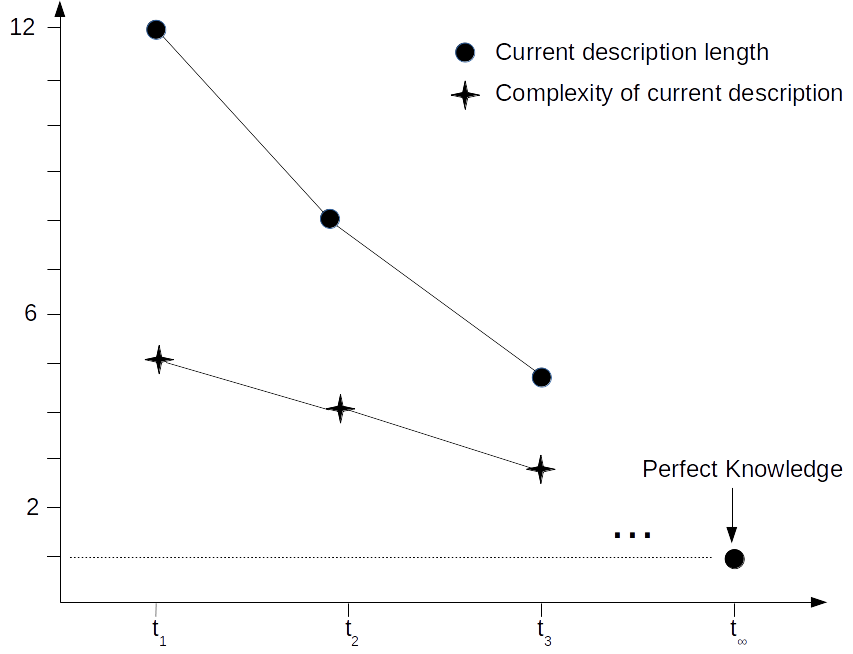
\includegraphics[scale=0.5]{Perfect_Knowledge}
\caption{\label{fig:Perfect_Knowledge}In Pursuit of Perfect Knowledge}
\end{figure}

{\color{red} TODO: Introduce the following definition.}

\begin{definition}
Let $s_{1}, \ldots, s_{n} \in T$ a collection of topics. The \emph{joint nescience} of topics topics $s_{1}, \ldots, s_{n}$ given the current best descriptions $\hat{d_{s_1}}, \ldots, \hat{d_{s_n}}$ is defined as: 
\[
{\color{red} TODO}
\]
\end{definition}

{\color{red} TODO: Mention, or prove, the properties of the generalized nescience}

%
% Current Best Description
%

\section{Current Best Description}

{\color{red} TODO: Rewrite this section}

We are also interested in our current understanding of the concatenation of two topics.

\begin{definition}
Given $t,s \in \mathcal{T}$ two different topics, and the set $\mathcal{D}_{t,s} = \{ d \in \mathcal{B}^\ast, d = \langle TM,a \rangle : TM(a) = \langle t,s \rangle \}$, let $\hat{d}_{t,s}$ be a distinguished element of $\mathcal{D}_{t,s}$. We call $\hat{d}_{t,s}$ our \emph{current best joint description} of $t$ and $s$.
\end{definition}

The concept of best joint description could be a little bit misleading, since given that the concatenation of any two topics is another topic, we could ask ourselves why do not simply use our current best description of the topic represented by that concatenation. That would make sense only in case that somebody has already studied both topics together. However, for the overwhelming majority of the possible combinations of topics, nobody has studied them yet.

\begin{example}
\label{ex:unknown_join}
Let $t$ and $s$ two different topics, and assume that nobody has studied them together before. In this case, our current best description $\hat{d}_{t, s}$ would be $\langle TM, \langle \hat{d}_t, \hat{d}_s \rangle \rangle$, where $TM$ is a Turing machine that given the input $\langle \hat{d}_t, \hat{d}_s \rangle$ prints out the string $ts$. If $\hat{d}_t = \langle TM_t, a_t \rangle$ and $\hat{d}_s = \langle TM_s, a_s \rangle$, the machine $TM$ will decode $\hat{d}_t$, run $TM_t(a_t)$ to print out $t$; then it would do the same for $\hat{d}_s$ to print $s$.
\end{example}

As we said in the preface of this chapter, in order to compute how much we do not know about a topic, first we need a way to quantify what we already know about that topic. How much we know about a topic will be given by our current best known description of that topic.

\begin{definition}
Given the set of descriptions $\mathcal{D}_t$ of a topic $t \in \mathcal{T}$, let $\hat{d_{t}}$ be a distinguished element of $\mathcal{D}_t$. We call $\hat{d_{t}}$ our \emph{current best description} of $t$.
\end{definition}

Which description is the current best description is something that depends on our current knowledge about the particular area in which the theory of nescience is being applied.


%
% Section: Nescience based on Datasets
%

\section{Nescience based on Datasets}
\label{sec:nescience_datasets}

{\color{red} TODO: Perhaps we should remove this section}

Some topics can be described unsing a mathematical model that can
be evaluated by a computer. For those topics we could estimate their
complexity using a sample dataset, for example the result of an experiment.
This property allow us, among other things, to compare how well topics
are described by different models (see Chapter \ref{chap:Structured-Datasets}).

\begin{definition}
Let $t\in T$ be a topic, $D=\left\{ x_{1},x_{2},\ldots,x_{n}\right\} $
the result of running an experiment that describes $t$, and $H$
a mathematical hipothesis for $t$. The complexity of the topic $t$
given the current description $H$ and the dataset $D$ is given by

\[
\hat{C}_{t}=L(H)+L(D\mid H)
\]
as it is described by the minimum description length principle.
\end{definition}

Given the dataset $D$ and the model $H$ we can compute our current
nescience of a topic as it is described by the next definition.

\begin{definition}
Let $t\in T$ a topic, $D=\left\{ x_{1},x_{2},\ldots,x_{n}\right\} $
the result of running an experiment that describes $t$, $C$ a code
that minimizes the length of $D$, and $H$ a mathematical hipothesis
for $t$. The current complexity of the topic $t$ given the dataset
$D$ and the hyphotesis $H$ is given by

\[
N_{t}=\frac{\hat{C_{t}}-l_{C}(D)}{l_{C}(D)}
\]

\end{definition}

In practice, the dataset $D$ also allows us to approximate our current
nescience of a topic $t$, given the model $H$. What we have to do
is to use a near minimal encoding for $D$, for example, by using
a Huffam encoding.


%
% Section
%

\section{Unknonwn Unknown}

{\color{red} TODO: pending}

Knonw unknown

Unknown unknown

Finally, there exists a last category of unknonw, what we call the unknowable unknown unknown. This category refers to those entities we

Unknowable unknown unknonwn. In this book we are interested in the unknown unknown

%
% Section: References
%

\section*{References}

{\color{red} TODO: Add the paper of Chaitin about the Berry paradox}

{\color{red} TODO: That there are numbers that are not computable can be found in the original paper of Turing}

{\color{red} TODO: Perhaps Ii should provide a couple of references in epistemology and ontology}
